% Load LaTeX and package
\documentclass[11pt, xcolor=x11names,compress]{beamer}
\usepackage[utf8]{inputenc}
\usepackage{mathtools}  % for paired delimiters 
\usepackage{mathrsfs}   % for script capitals
\usepackage{amsmath}
\usepackage{amssymb}
\usepackage{amsfonts}

\usepackage[dvipsnames]{xcolor} % for color
\usepackage{ragged2e} % for text alignment
\usepackage{dsfont} % for sepecial font (mathds)

\usepackage[labelformat=empty]{caption}

\usepackage{natbib}
\bibliographystyle{abbrvnat}
% Customize theme attributes
\setbeamertemplate{headline}[default]
%% Hide navigation symbols
\setbeamertemplate{navigation symbols}{}
%%\mode<beamer>{\setbeamertemplate{blocks}[rounded][shadow=true]} %for block
%% Outer theme
\useoutertheme{infolines}
\useoutertheme[subsection=false]{miniframes}

%% Inner theme
\useinnertheme{}

% Define template colors
\usecolortheme{rose}
%\usecolortheme{default}

\definecolor{UniColor}{RGB}{0,0, 255}
\setbeamercolor{structure}{bg=white, fg=UniColor}
\setbeamercolor{title}{bg = white, fg = UniColor}
\setbeamercolor{author}{bg = white, fg = UniColor}

\DeclareMathOperator{\Var}{\text{Var}}
\DeclareMathOperator{\E}{\text{E}}
\DeclareMathOperator{\Cov}{\text{Cov}}
\DeclareMathOperator{\Corr}{\text{Corr}}

%------------------------------------------------------------
%This block of code defines the information to appear in the
%Title page


\title [ECON 4003: Introduction to STATA]{ECON 4003 Econometrics I}

\vspace{10mm}

\author[]{Introduction to STATA}
\date{}

%End of title page configuration block
%---------------------------------------------------- 

\begin{document}
\setbeamertemplate{caption}[numbered]
%The next statement creates the title page.
{\titlegraphic{
\includegraphics[scale = 0.05]{GlaLogo.pdf}}
\frame{\titlepage}}

%---------------------------------------------------------

\begin{frame}[fragile,t]
\linespread{1.3}
\frametitle{About Lab Sessions}
\begin{itemize}
    \item 9 hours tutor-led computing sessions (6 x 1.5 hour): Week 3, 6-10
    \item GOAL: Use statistical software (Stata) to perform econometric analysis on empirical data
    \item Download and have a look at materials (exercises and datasets) from Moodle page in advance

\end{itemize}


\end{frame}
%---------------------------------------------------------

%---------------------------------------------------------

\begin{frame}[fragile,t]
\linespread{1.3}
\frametitle{Overview - Introduction to Stata}
\begin{itemize}
    \item Little or no previous experience in Stata before
    \item Learning Objectives:
    \begin{itemize}
        \item Familiarise yourself with the Stata interface
        \item Set the working directory and get data in and out of Stata
        \item Perform basic data analysis: Data Description, Graphics, Data Management
    \end{itemize}

\end{itemize}


\end{frame}
%---------------------------------------------------------


%---------------------------------------------------------
\begin{frame}[fragile,t]
\frametitle{What is Stata? Statistics and Data Analysis}
\begin{itemize}
    \item A statistical package that includes a wide variety of capabilities
    \begin{itemize}
        \item Data management
        \item Statistical and econometric analysis
        \item Graphics etc.
    \end{itemize}
    \item Widely used in the fields of economics, finance, political science, sociology, biomedicine and epidemiology
    \item Three main versions
    \begin{itemize}
        \item Stata/IC (Intercooled): mid-sized datasets
        \item Stata/SE (Special Edition ): large datasets
        \item Stata/MP (Multi-processor ): fastest version (for quad-core, dual-core, and multicore/multiprocessor computers)
    \end{itemize}
\end{itemize}
\end{frame}
%---------------------------------------------------------

%---------------------------------------------------------
\begin{frame}[fragile,t]
\frametitle{Stata Interface}
\begin{figure}
    \centering
    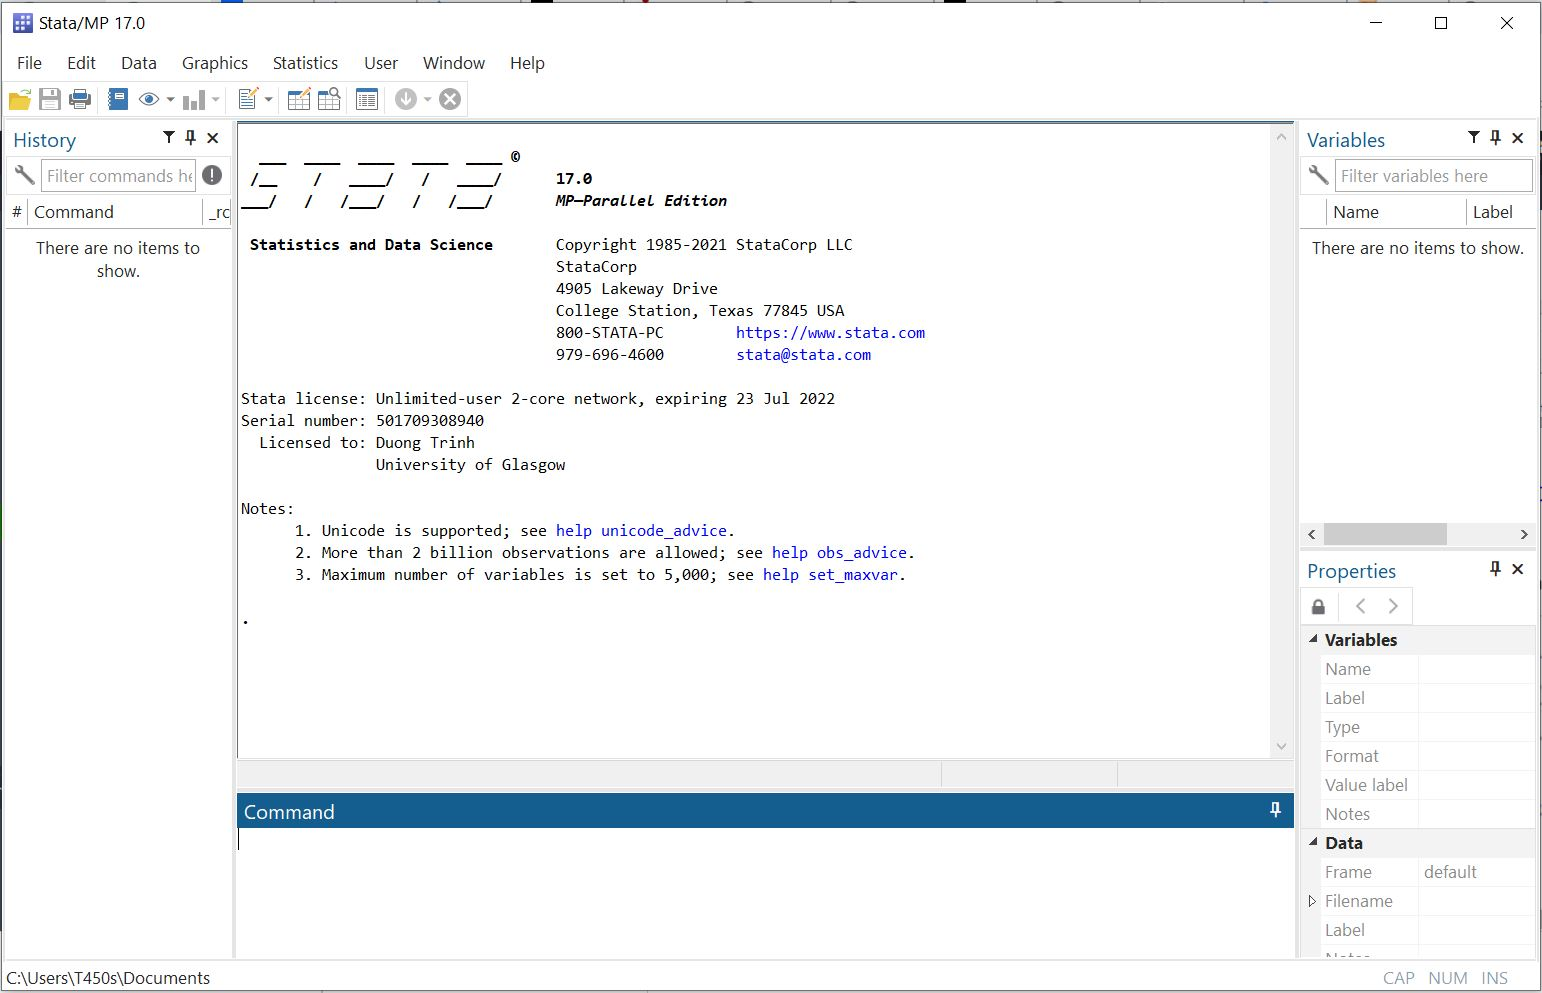
\includegraphics[scale = 0.35]{StataIterface.JPG}
    \caption{}
    \label{fig:my_label}
\end{figure}
\end{frame}
%---------------------------------------------------------

%---------------------------------------------------------
\begin{frame}[fragile,t]
\frametitle{Stata Interface: Command Window}
\begin{figure}
    \centering
    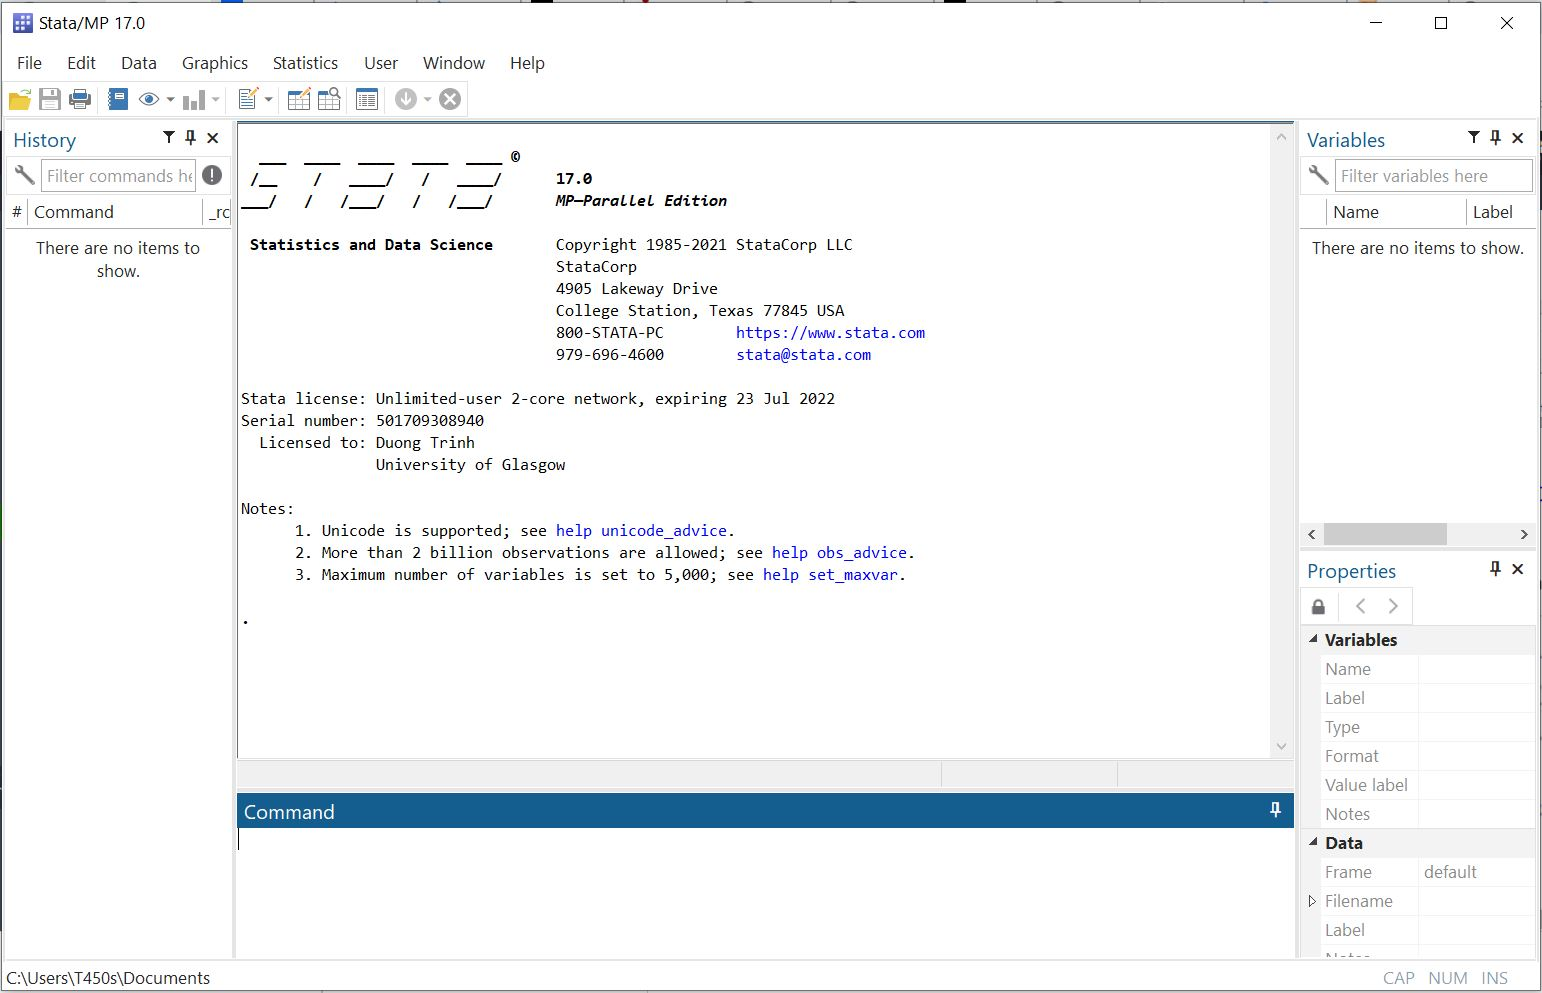
\includegraphics[scale = 0.35]{StataIterface.JPG}
    \label{fig:my_label}
    \caption{Type the instructions we want Stata to execute}
\end{figure}
\end{frame}
%---------------------------------------------------------

%---------------------------------------------------------
\begin{frame}[fragile,t]
\frametitle{Stata Interface: Results Window}
\begin{figure}
    \centering
    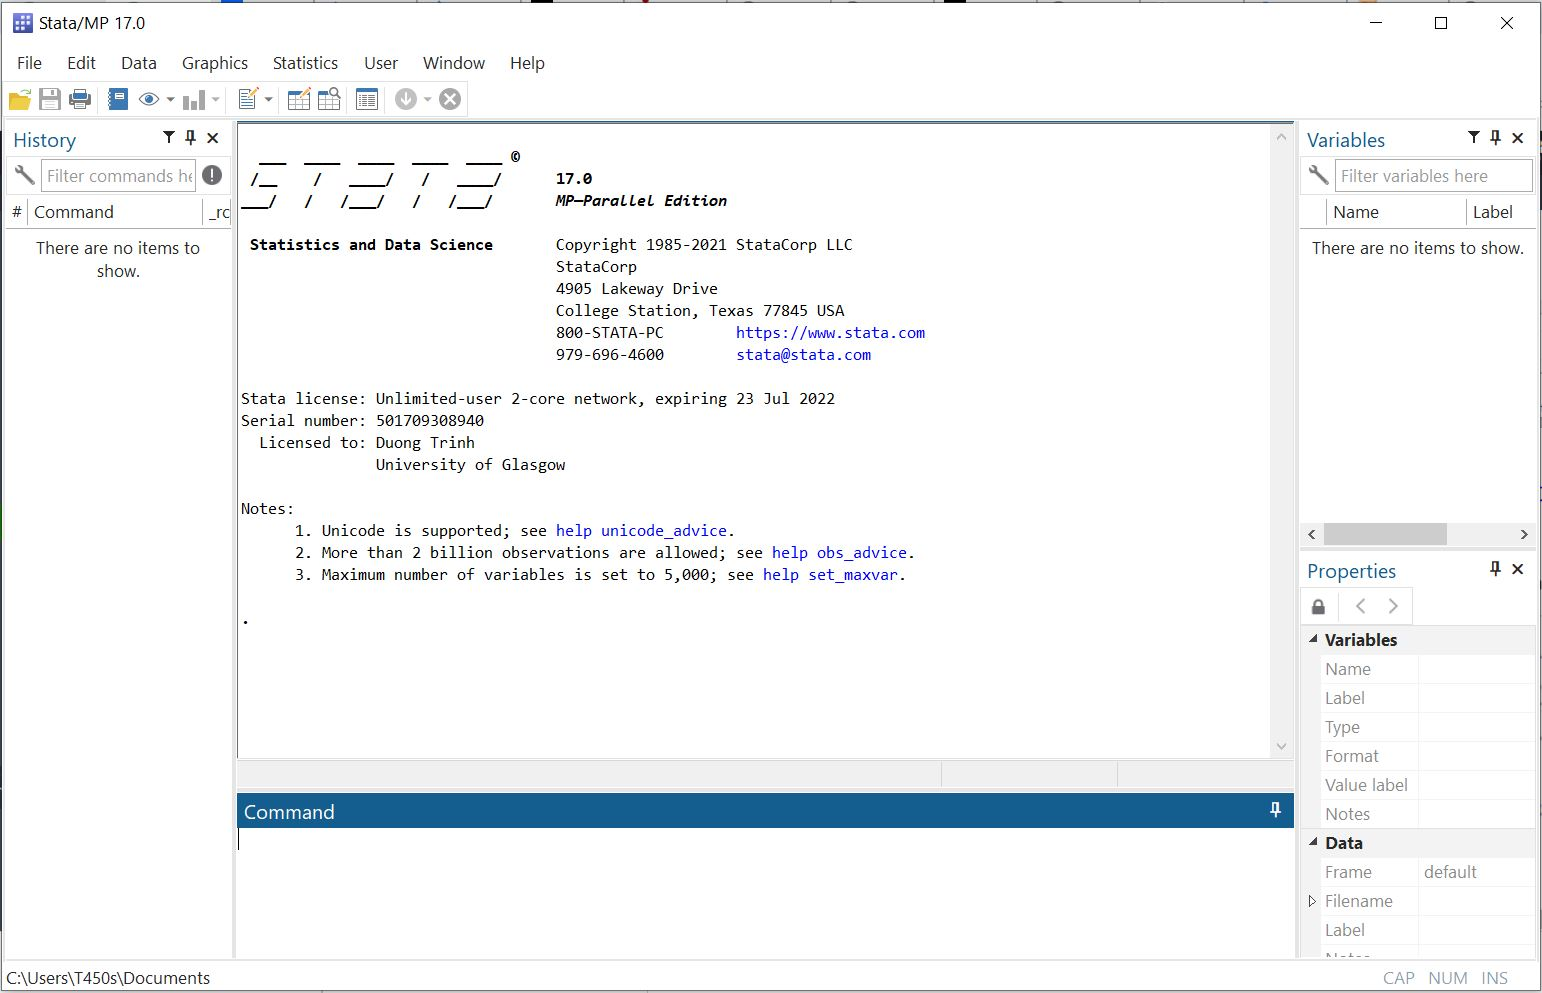
\includegraphics[scale = 0.35]{StataIterface.JPG}
    \label{fig:my_label}
    \caption{Displays the results and outputs after a command is executed}
\end{figure}
\end{frame}
%---------------------------------------------------------

%---------------------------------------------------------
\begin{frame}[fragile,t]
\frametitle{Stata Interface: Review Window}
\begin{figure}
    \centering
    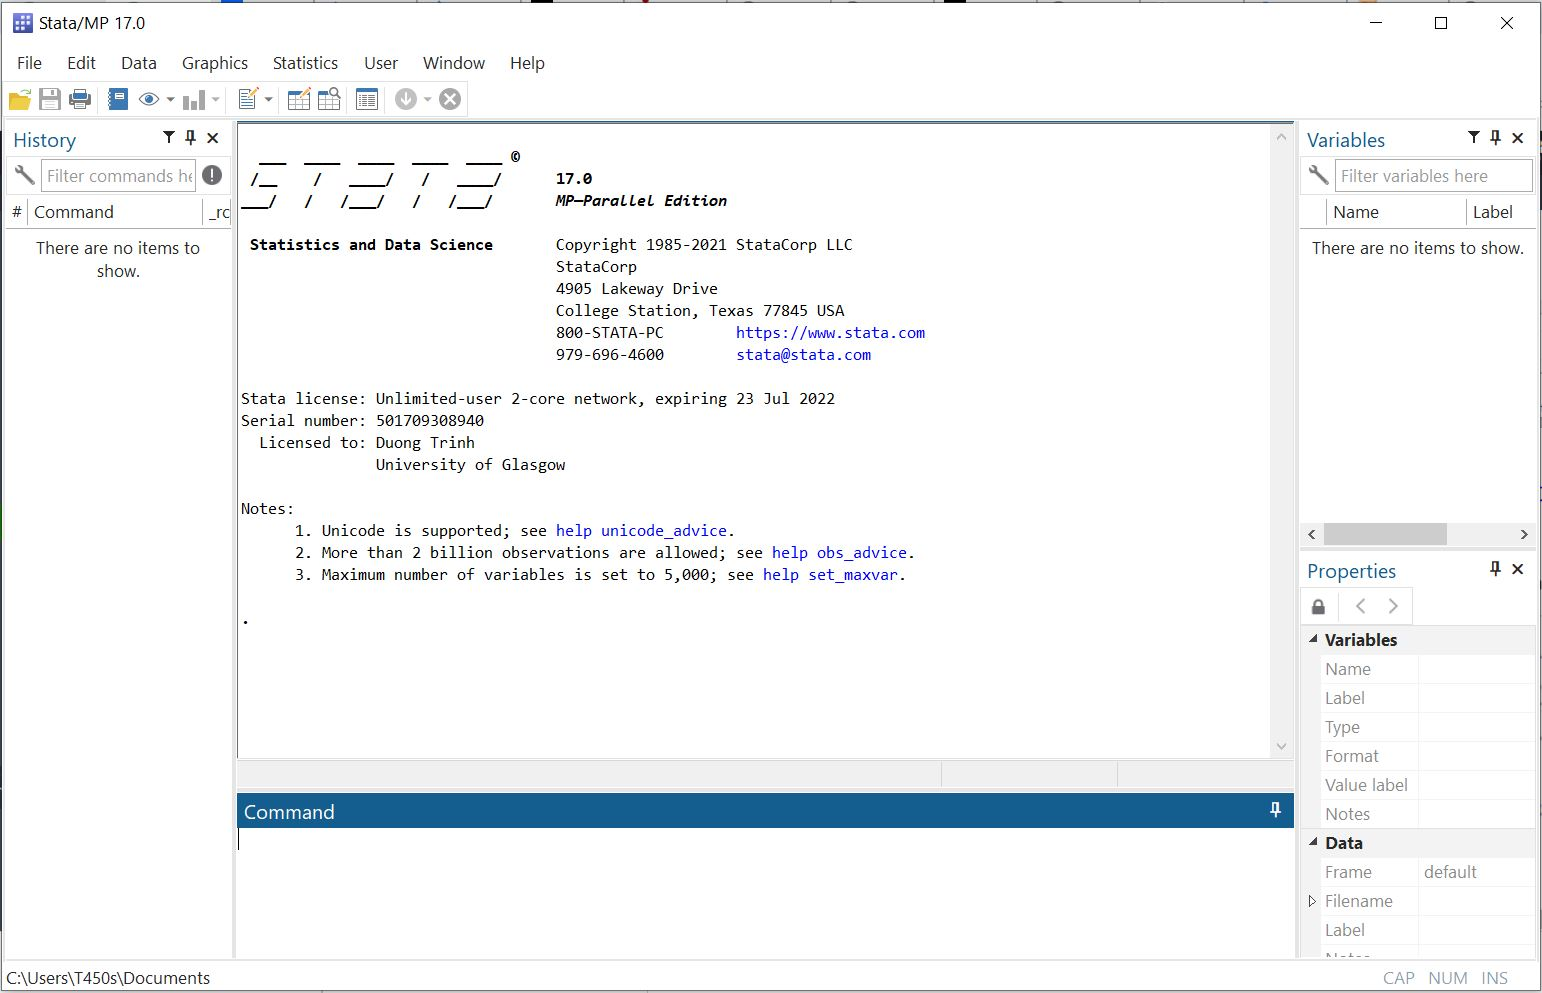
\includegraphics[scale = 0.35]{StataIterface.JPG}
    \label{fig:my_label}
    \caption{Keeps a record of all the commands used/the input history}
\end{figure}
\end{frame}
%---------------------------------------------------------

%---------------------------------------------------------
\begin{frame}[fragile,t]
\frametitle{Stata Interface: Variables Window}
\begin{figure}
    \centering
    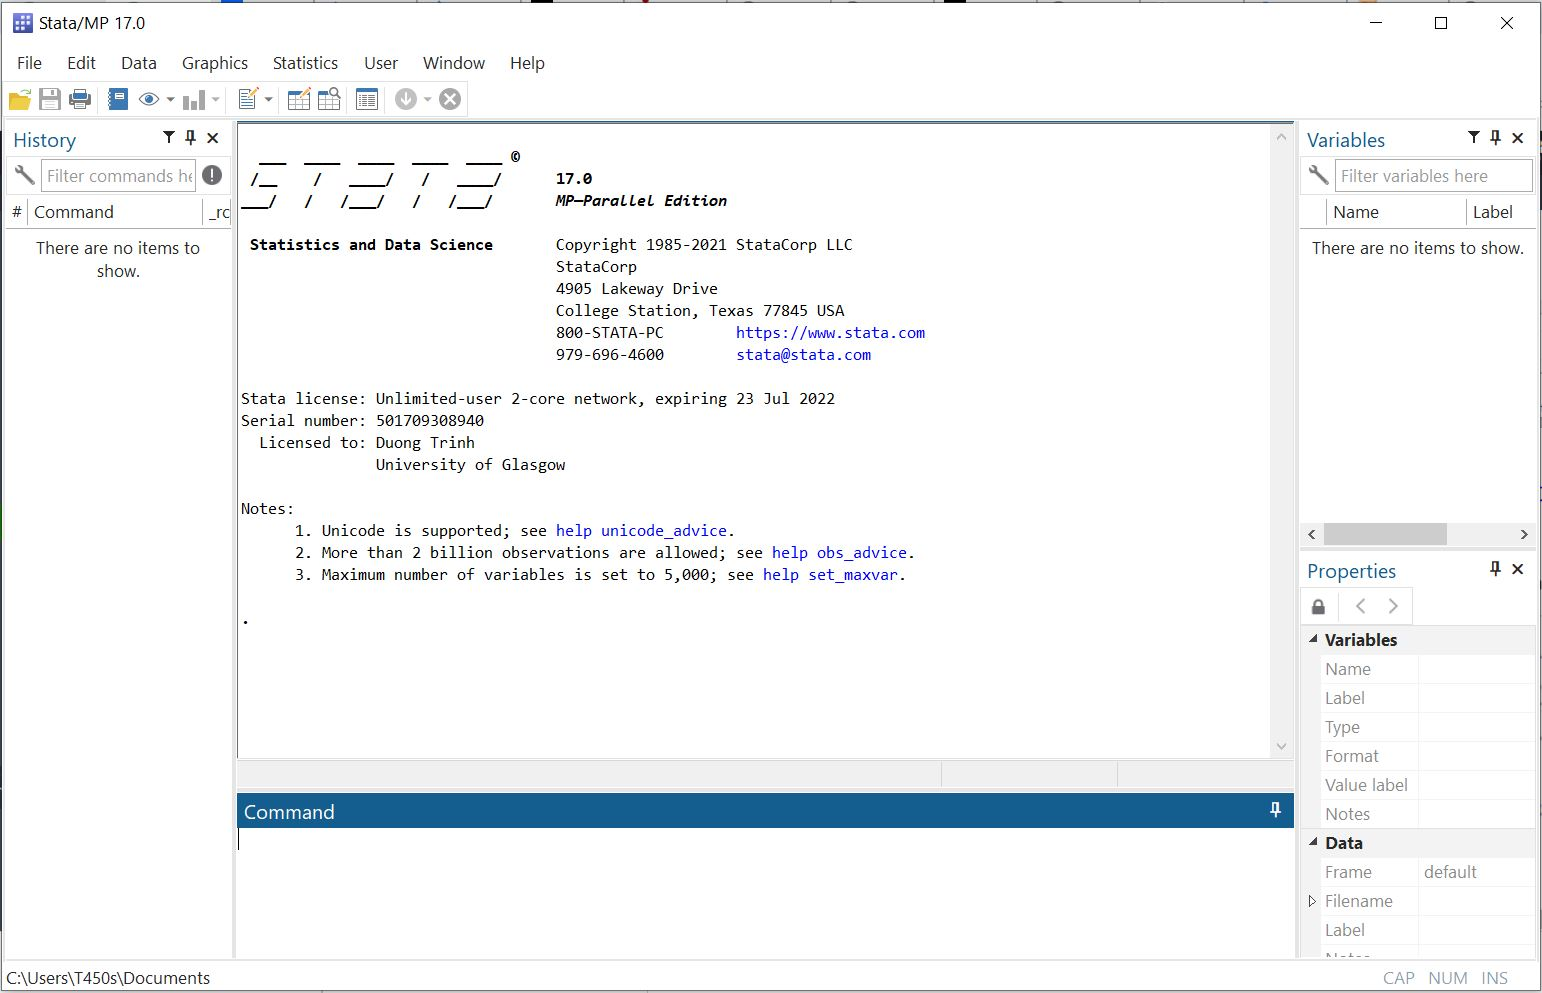
\includegraphics[scale = 0.35]{StataIterface.JPG}
    \label{fig:my_label}
    \caption{Shows all the variables in the dataset}
\end{figure}
\end{frame}
%---------------------------------------------------------

%---------------------------------------------------------
\begin{frame}[fragile,t]
\frametitle{Stata Interface: Properties Window}
\begin{figure}
    \centering
    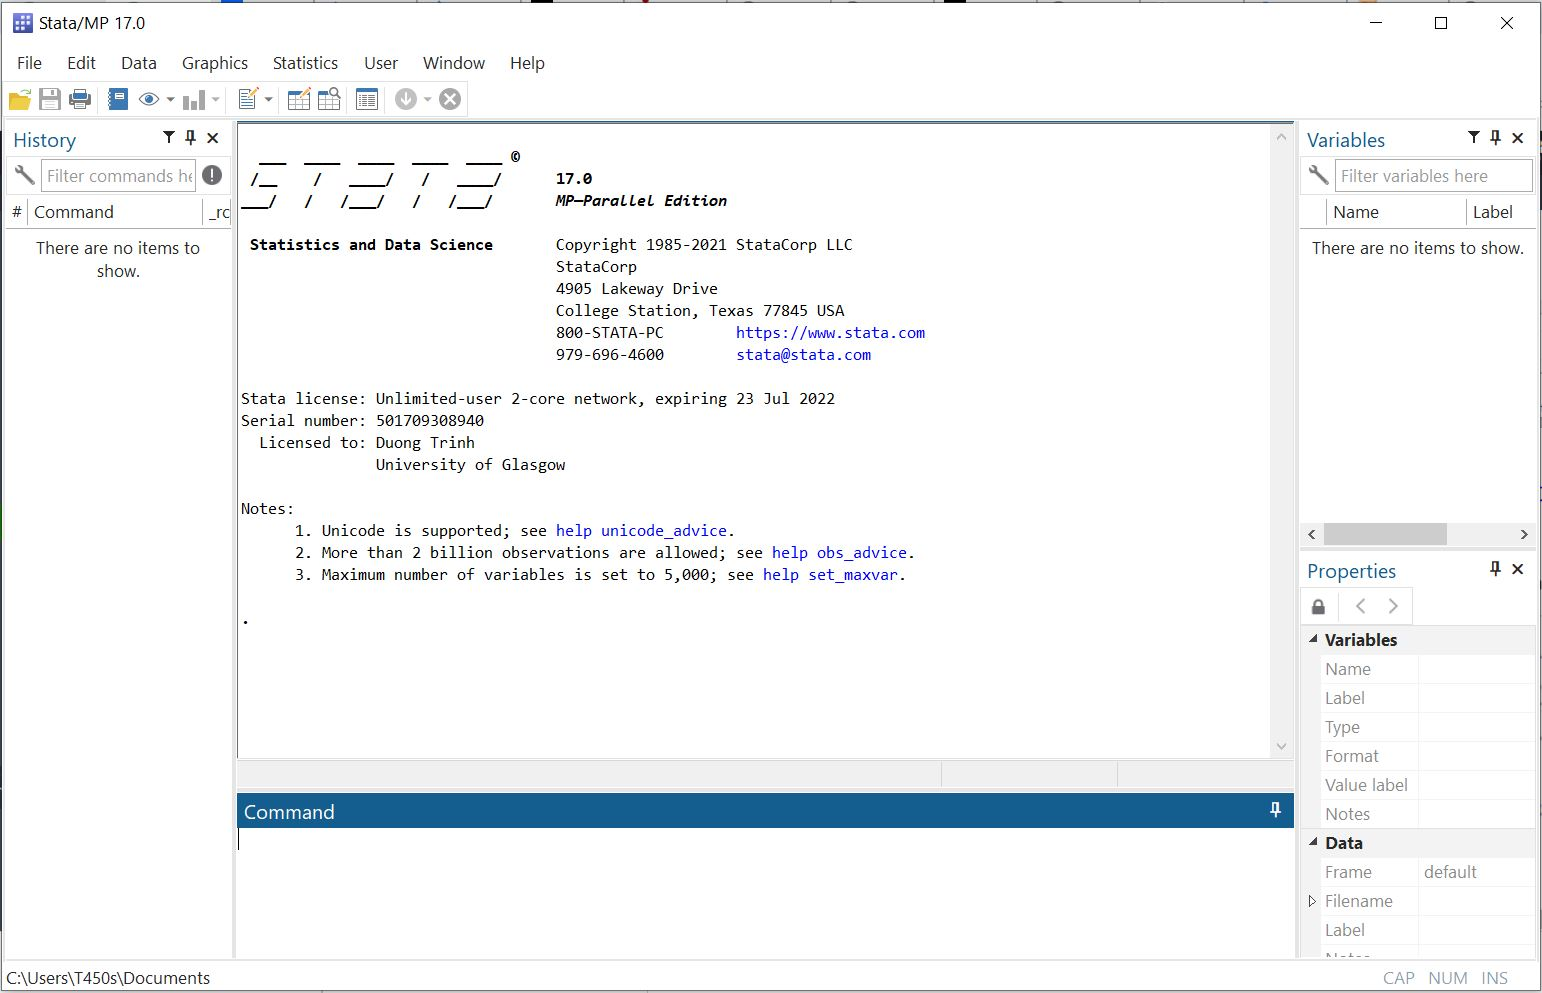
\includegraphics[scale = 0.35]{StataIterface.JPG}
    \label{fig:my_label}
    \caption{Indicates the properties of a highlighted variable}
\end{figure}
\end{frame}
%---------------------------------------------------------

%---------------------------------------------------------
\begin{frame}[fragile,t]
\frametitle{Stata Interface: Current Working Directory}
\begin{figure}
    \centering
    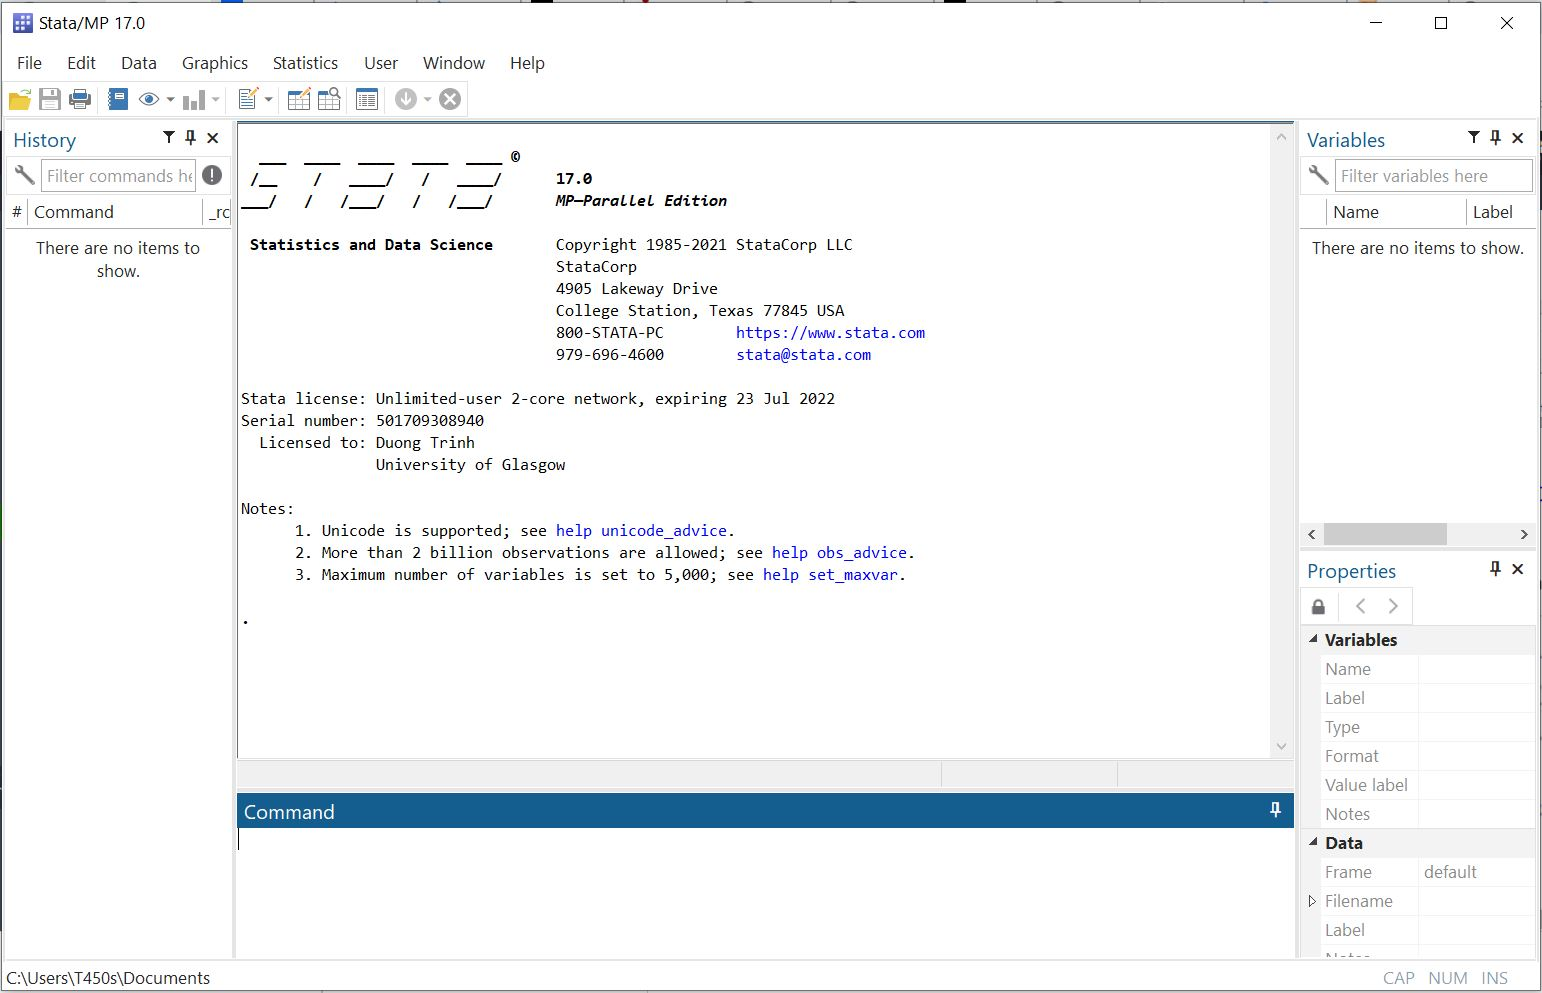
\includegraphics[scale = 0.35]{StataIterface.JPG}
    \label{fig:my_label}
    \caption{Shows current directory in file system from where Stata will read or save any file}
\end{figure}
\end{frame}
%---------------------------------------------------------

%---------------------------------------------------------
\begin{frame}[fragile,t]
\frametitle{Stata Characteristics}
\begin{itemize}
    \item Basic syntax:
    \begin{center}
        $\texttt{command}$ varlist , options
    \end{center}
    \item Relational operations
    \begin{itemize}
        \item $>$ greater than
        \item $<$ less than
        \item $>=$ greater than or equal
        \item $<=$ less than or equal
        \item $==$ equal
        \item $!=$ not equal
    \end{itemize}
    \textcolor{red}{(!)CAUTION} $=$ is NOT equal to $==$
    \item Logical operators 
    \begin{itemize}
        \item $\&$ and
        \item $|$ or
        \item $!$ not
    \end{itemize}

\end{itemize}
\end{frame}
%---------------------------------------------------------

%---------------------------------------------------------
\begin{frame}[fragile,t]
\frametitle{Stata Characteristics}
\begin{itemize}
    \item Mathematical operations
    \begin{itemize}
        \item $+$ addition
        \item $-$ subtraction
        \item $*$ multiplication
        \item $/$ division
        \item $\wedge$ exponentiation
    \end{itemize}
    \item Use $*$ for \textcolor{green}{comments}
    \item Use $""$ for \textcolor{brown}{strings}
    \item Capitalization consistency
    \begin{itemize}
        \item Stata is sensitive to capitalized words for variables
        \item Stata does not understand capitalized commands 
    \end{itemize}
\end{itemize}
\end{frame}
%---------------------------------------------------------

%---------------------------------------------------------
\begin{frame}[fragile,t]
\frametitle{PRACTICE: Data Description}
*Ex1: which is the mean of the variable tenure for those women who live in the south?

\vspace{5mm}

*Ex2: which is the working hour’s mean for married women who belong to a union?

\vspace{5mm}

*Ex3: is it higher or lower than the working hours average of single women who belong to a union?

\vspace{5mm}

\end{frame}
%---------------------------------------------------------

%---------------------------------------------------------
\begin{frame}[fragile,t]
\frametitle{PRACTICE: Graphics}
*Ex1: draw pie chart for “occupation”

\vspace{5mm}

*Ex2: create a bar graph for the variable “married”

\vspace{5mm}

*Ex3: create a horizonal bar graph for the variable “industry”

\vspace{5mm}

*Ex4: repeat the hist exercise above for the variable “hours”

\vspace{5mm}

*Ex5: create a scatter plot of “wage” on “ttl\_exp”

\vspace{5mm}

*Ex6: create a scatter plots of “wage” on “ttl\_exp” by “married"

\end{frame}
%---------------------------------------------------------

%---------------------------------------------------------
\begin{frame}[fragile,t]
\frametitle{PRACTICE: Data Management}
*Ex1: create a new variable called “totwage” which is “wage” multiplied by “hours”. 

\vspace{5mm}

*Ex2: replace “totwage” with the natural log of “totwage”? (hint: natural log of x is “log(x)”).  

\vspace{5mm}

*Ex3: what is the mean of "totwage"?

\end{frame}
%---------------------------------------------------------


\end{document}